\documentclass[sigconf]{acmart}

\usepackage{graphicx}
\usepackage{hyperref}
\usepackage{todonotes}

\usepackage{endfloat}
\renewcommand{\efloatseparator}{\mbox{}} % no new page between figures

\usepackage{booktabs} % For formal tables

\settopmatter{printacmref=false} % Removes citation information below abstract
\renewcommand\footnotetextcopyrightpermission[1]{} % removes footnote with conference information in first column
\pagestyle{plain} % removes running headers

\newcommand{\TODO}[1]{\todo[inline]{#1}}

\begin{document}
\title{Big DATA IN RAIN WATER HARVESTING}


\author{Rahul Velayutham}
\affiliation{%
  \institution{Indiana University Bloomington}
  \streetaddress{2661 H 7th St}
  \city{Bloomington} 
  \state{Indiana} 
  \postcode{47408}
}
\email{rahuvela@umail.iu.edu}

% The default list of authors is too long for headers}
\renewcommand{\shortauthors}{R. Velayutham}


\begin{abstract}
Big Data is rapidly becoming a crucial component in the majority of the fields, be it from medicine to software. Big data technologies help in processing humongous amounts of data in a rapid manner while enabling us to achieve results fast and accurately. Big data is becoming a key player in the restoration of ecological assets like water, forests and the likes. Real time analysis of assets all over the world and the changes are documented and stored how this data can be used and for what purpose is the penultimate question. We dissect the various stages of the rainwater harvesting process and show how the application of big data to each stage can enhance the process.
\end{abstract}

\keywords{Big Data, i523 , HID 232 , Rain Water Harvesting}


\maketitle



\section{Introduction}

Rainwater harvesting is the accumulation and deposition of rainwater for reuse on-site, rather than allowing it to run off. Rainwater can be collected from rivers or roofs, and in many places, the water collected is redirected to a deep pit (well, shaft, or borehole), a reservoir with percolation, or collected from dew or fog with nets or other tools. Its uses include water for gardens, livestock, irrigation, domestic use with proper treatment, indoor heating for houses, etc. The harvested water can also be used as drinking water, longer-term storage, and for other purposes such as groundwater recharge.Rainwater harvesting is one of the simplest and oldest methods of self-supply of water for households usually financed by the user. \cite{Wikipedia2016}. Rainwater harvesting is also used to tackle the problem of water scarcity. Water scarcity caused due to pollution, global warming and overuse has become a huge threat to the existence of man. solving this simply by filtration and redistribution of water from dams and from normal rainfall, these can be augmented with rainwater harvesting systems. 

\section{Big data in rain water harvesting}

\subsection{Introduction}
Before the subject matter of big data in rainwater harvesting is tackled it is first necessary to understand the rainwater harvesting process before the combination with big data can be explained. For the purpose of this study, the method rooftop rainwater harvesting is used. In brief, the rainwater harvesting process can be grossly oversimplified as follows:
\begin{itemize}
  \item Analyze feasibility of installation
  \item Installation
  \item First wash
  \item route rainwater to storage tank
  \item redirect water in case of overflow
\end{itemize}
the figure \ref{f:water} provides a good explanation on rainwater harvesting process
\begin{figure}[!ht]
  \centering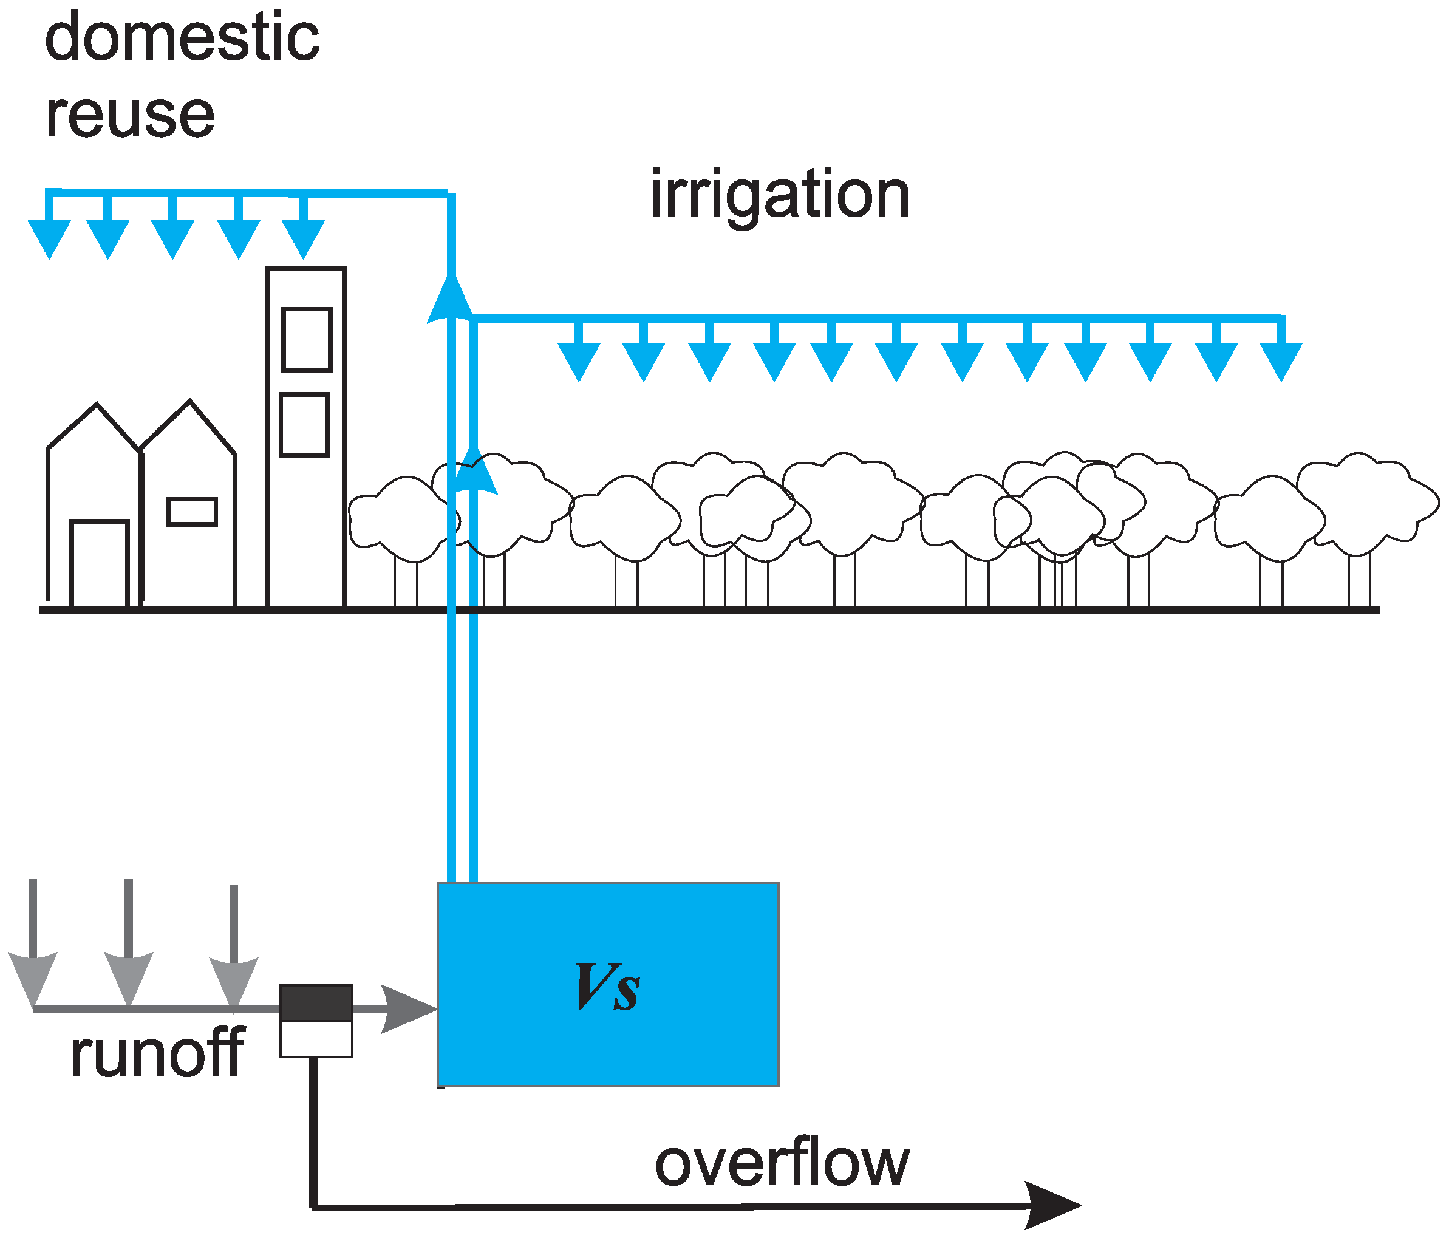
\includegraphics[width=\columnwidth]{images/water.pdf}
  \caption{rainwater harvesting figure}\label{f:water}
\end{figure} 
and a good article to explain the rainwater harvesting process can be found here \cite{Wikipedia2016}. The first wash step, in particular, is very important because it removes dust debris etc from the rooftop or else we risk contamination of water. Quite naturally we cannot allow the collected rainwater to overfill tanks in case of this we need to redirect the water to some other outlet.Big data can play a very influential role right from the feasibility analysis to re direction of water.

\subsection{Big data and feasibility of installation}
Big data can play a huge role in the feasibility estimation. This can be useful for both households and governments, in many countries in some states it is mandatory that each house should have a rainwater harvesting unit. In some cases, these are funded by the government and in some cases it in on the owner to do so. In the case of governments to do an analysis how can they do so, it is a huge task to go to each and every house and track roof dimensions. One easy way of going about this would be to use satellite image data. These images can then be searched for roof features and dimensions accordingly extrapolated and in such a manner the dimensions of many roofs can be obtained and a cost estimate can be obtained. To obtain the data we can use the many datasets provided by NASA or we can even use a highly zoomed street view from google maps. To extract the features we can use one of the many open CV libraries or use apply complex ML deep learning algorithms . To store this data a simple Hadoop map-reduce can be used. A more detailed study can be viewed in \cite{RobertO.Ojwang2015}.

\subsection{Big data and first wash}
the importance of first wash was previously stressed upon in the introduction. it is required to wash away dust, debris, dead insects and other such contaminants. The first watch is a manual task it is dependent on the owner to redirect the first wash water elsewhere. Often most people have mistaken it to be the first wash to be the first rain, that is people waste a whole day of rain at times as first wash, or some mistakenly use small drizzles as the first and do not use the first watch properly. Big data can help in the automation of the first wash process combined with IoT. The first step would be to obtain the weather data, this can be achieved either by using the highly consolidated data obtained from the respective government's  meteorology departments or the huge datasets provided by the NASA satellite. Once again Hadoop map-reduce allows for reducing a humongous data set into more compact usable structures. From this we can perform a weather data analysis to determine if the rain will be heavy/light and its duration. From this data, we can easily determine when to perform the first watch. Assuming every rainwater harvesting unit has an IoT feature that controls the valves or water redirection one central control center can send signals to a wide area on when to perform the first watch and for how long. This should greatly reduce the amount of rainwater wasted.

\subsection{Big data and water tanks}
Big data and IoT can once again help in the rainwater harvesting process, there are many times water left in the tanks are not used and the water becomes stagnant with the use of devices the quality of water can be checked and the tanks can be drained. Also, it is very difficult to combine the rainwater tanks with the main water channels of the buildings since the water in the tanks is very very limited. With the help of IoT redistributing this water becomes very easy using data from other parts of the housing analysis can be made water can be redistributed accordingly. Then there is also the matter of making sure the tanks don't overflow which could lead to bursting. Using IoT the water can be tracked in a smart manner and decisions like when to reroute can be done in a smart manner. There is one more important use for big data in tanks, leakages and rusting. As previously mentioned the quality of water can be checked by its ph level using smart devices the next issue comes down to leakages. more often than not most installations are buried under the ground this is done in order to reduce the effects of weather and also so that the installation doesn't take up space. While this leads to a new set of problems the major one is that often leaks cant be detected until its too late. IoT devices can be used to alert a user that water levels are falling down way too rapidly and the user can contact servicemen in time before the next rains.

\subsection{Big data and water re routing}
Lastly but perhaps most important is the issue of rerouting water once the tanks get full. In the majority of the cases, the rainwater is directly diverted to the water table. While it is normally a good idea to replenish the water table in such a manner due to over exploitation from bore wells. Aside from restoring the water table, it is slowly becoming essential to recharge even the lakes and other sources of freshwater. This is becoming important because with global warming and rainfall becoming more erratic [ some places receiving more rainfall than the others and others receiving way lesser] as a result we need to divert some of the harvested rainwater to other lakes/reservoirs. As to how this can be achieved we can use Big data to monitor the water levels and then decide accordingly where to route the rainwater and by how much.

\section{Tech in rain water harvesting}
Surprisingly there is not much to write about about very few players exist in the rainwater harvesting market who aim to offer the services of big data. Part of this can be attributed to the fact there is not much data available. For example, Indian government offers highly consolidated annual precipitation data for free while this is useful to perform past estimates it however is really not enough, more detailed minute by minute data of precipitation is required in order for the above mentioned analysis to take place. Even the NASA weather data doesn't give the whole picture. This doesn't mean the data is not there but a premium is required to obtained it. there are a few players who offer smart tank service . However the tech scene is just getting  warmed up and awareness of its potential is doing rounds a good article was recently released by NASA on this \cite{Morrow2015} and a few examples are \cite{UNEP2017}.

\section{Conclusion}

The scope for big data in rainwater harvesting is immense but the major initative lives with the governments, rerouting water into reservoirs is not in the best interests of private contractors but they can be hired to make it so. This can create a huge job market and it will be beneficial for all involved. This also needs to be done sooner rather than later because the rate of population growth exceeds our available sources and if we want the future generations to have any resources we need to embrace technology and start protecting our assets. Also, for private contractors to approach the government with proposals it would be very useful if more relevant data was made available to the public and thus there is a need for investment in the weather department for data.Rainwater harvesting despite being one of the oldest practices of water replenishment is surprisingly behind in terms of technology advancement when we look at the progress made with solar and wind.


\begin{acks}

  The authors would like to thank Dr. Gregor von Laszewski for his support and suggestions to write this paper.

\end{acks}

\bibliographystyle{ACM-Reference-Format}
\bibliography{report} 

\appendix

\section{Issues}

\subsection{Formatting}

    \done{Incorrect number of keywords or HID and i523 not included in the keywords}
    \done{Other formatting issues: No introduction?}



\subsection{Details about the Figures and Tables}

    \done{Capitalization errors in referring to captions, e.g. Figure 1, Table 2}

\section{Bibtex Issues}
\done[inline]{Warning--no number and no volume in Bialik2014}
\done[inline]{Warning--page numbers missing in both pages and numpages fields in Bialik2014}
\done[inline]{Warning--no number and no volume in cooling}
\done[inline]{Warning--page numbers missing in both pages and numpages fields in cooling}
\done[inline]{Warning--no number and no volume in learnbigdataanalytics2000}
\done[inline]{Warning--page numbers missing in both pages and numpages fields in learnbigdataanalytics2000}
\done[inline]{Warning--no number and no volume in 2012}
\done[inline]{Warning--page numbers missing in both pages and numpages fields in 2012}
\done[inline]{Warning--no number and no volume in Luca20000}
\done[inline]{Warning--page numbers missing in both pages and numpages fields in Luca20000}
\done[inline]{Warning--no number and no volume in 2000}
\done[inline]{Warning--page numbers missing in both pages and numpages fields in 2000}
\done[inline]{Warning--no number and no volume in Optasports2000}
\done[inline]{Warning--page numbers missing in both pages and numpages fields in Optasports2000}
\done[inline]{Warning--no number and no volume in Outsideoftheboot2000}
\done[inline]{Warning--page numbers missing in both pages and numpages fields in Outsideoftheboot2000}
\done[inline]{Warning--no number and no volume in Ramasamy2000}
\done[inline]{Warning--page numbers missing in both pages and numpages fields in Ramasamy2000}
\done[inline]{Warning--no number and no volume in Rein2016}
\done[inline]{Warning--page numbers missing in both pages and numpages fields in Rein2016}
\done[inline]{Warning--no number and no volume in Rejec2000s}
\done[inline]{Warning--page numbers missing in both pages and numpages fields in Rejec2000s}
\done[inline]{Warning--no number and no volume in Tutorialspoint2000}
\done[inline]{Warning--page numbers missing in both pages and numpages fields in Tutorialspoint2000}
\done[inline]{Warning--no number and no volume in wikipedia}
\done[inline]{Warning--page numbers missing in both pages and numpages fields in wikipedia}
\done[inline]{(There were 26 warnings)}


\end{document}
